\documentclass[12pt, a4paper]{article}

\usepackage{makra}

\makeatletter
\newcommand{\linia}{\rule{\linewidth}{0.4mm}}
\renewcommand{\maketitle}{\begin{titlepage}

    \vspace*{1cm}
    \begin{center}\small
    Uniwersytet Gdański\\
    Wydział Matematyki, Fizyki i Informatyki
    \end{center}
    \vspace{3cm}
    \noindent\linia
    \begin{center}
      \huge \textsc{\@title}
         \end{center}
     \linia
    \vspace{0.5cm}

    \begin{flushright}
    \begin{minipage}{9cm}
    \textit{\large Autor:}\\
    \normalsize \textsc{\@author} \par
    \end{minipage}
    \vspace{5cm}\\\\\\\\\\\\\\
			\small Wkrocz w świat liczb...\\
     \end{flushright}
    \vspace*{\stretch{6}}
    \begin{center}
    \@date
    \end{center}
  \end{titlepage}
}

\makeatother
\author{Tomasz Kopka }

\title{Magia algebry liniowej}
\begin{document}
\maketitle
    \vspace*{1cm}
\tableofcontents

\begin{figure}
	\centering
		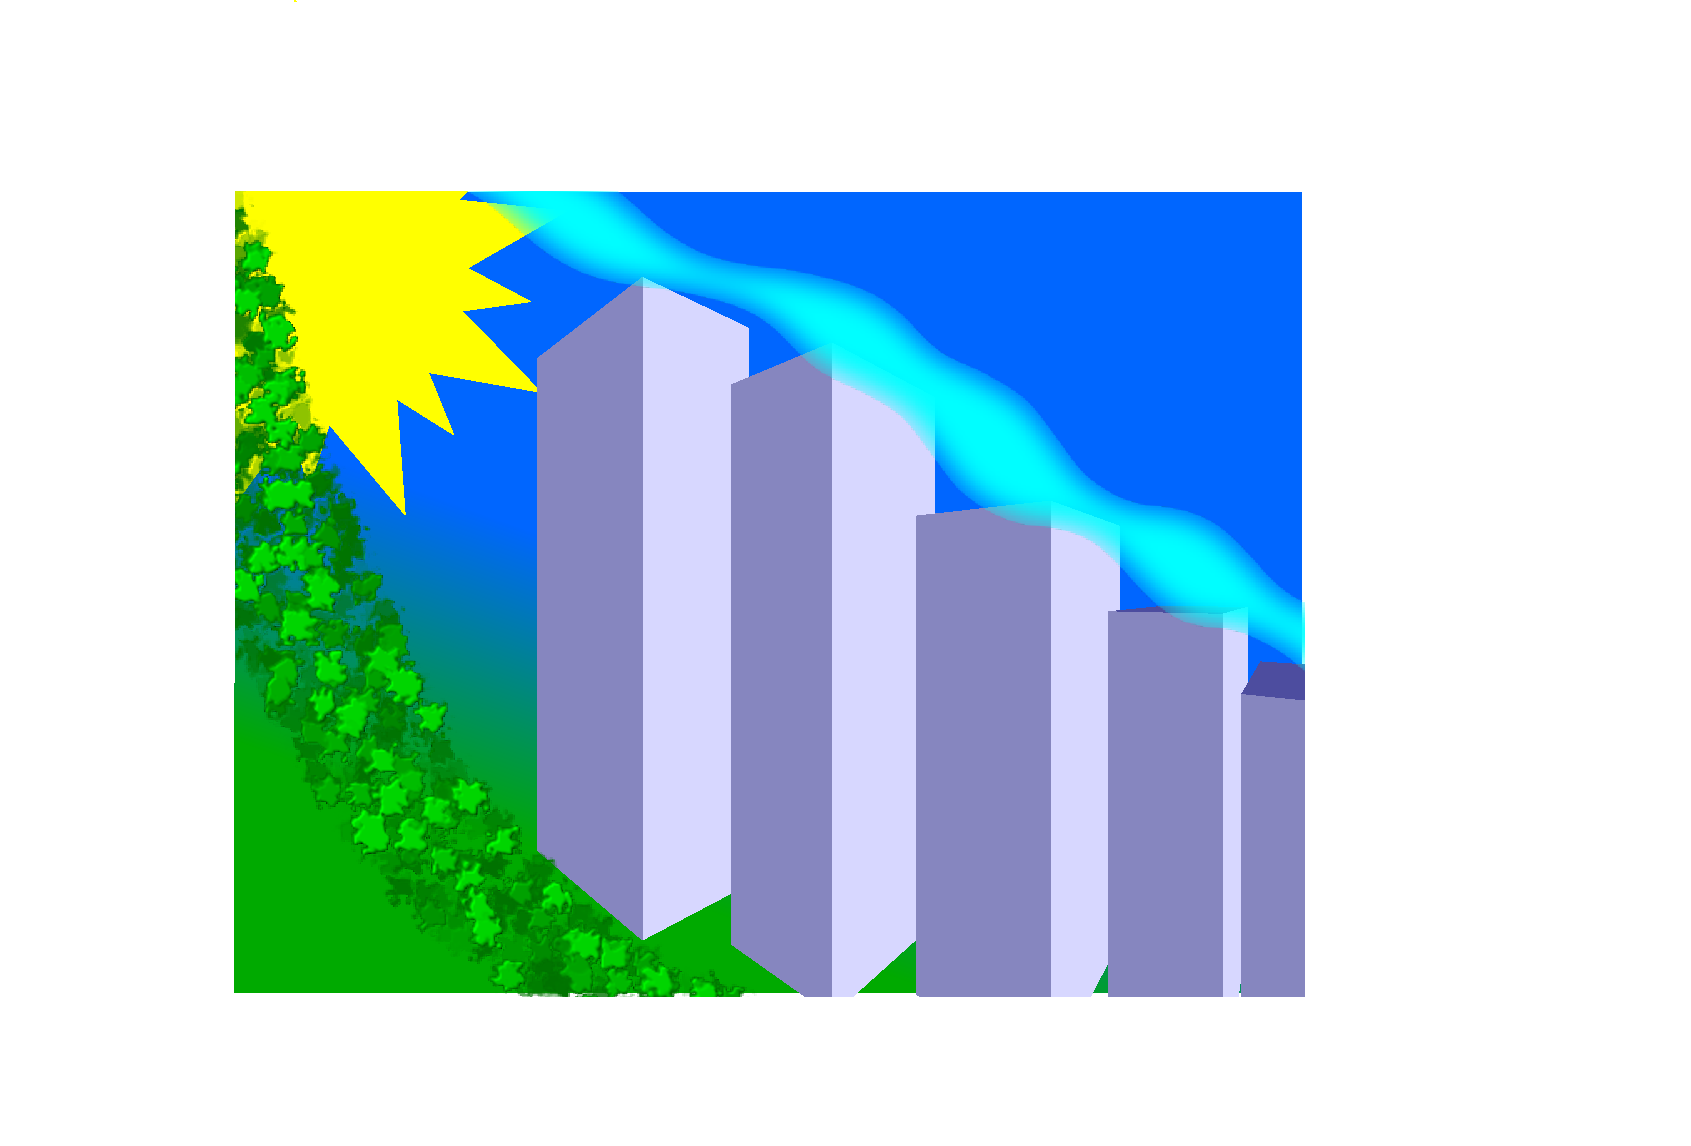
\includegraphics[width=0.90\textwidth]{Rysunek.pdf}
	\label{fig:Rysunek}
\end{figure}

\newpage
\section{Liczby zespolone}
\label{sec:Liczbyzespolone}
\subsection{Wstęp}
\label{sec:Wstep}

\subsubsection{Definicja}
\label{sec:Definicja}


\begin{center}\large {Liczby zespolone}
\end{center}
– liczby będące elementami rozszerzenia ciała liczb rzeczywistych o jednostkę urojoną $i$, tj. pierwiastek wielomianu $x^2+1$ (innymi słowy, jednostka urojona spełnia równanie $i^2 = -1$). Każda liczba zespolona z może być zapisana w postaci $z=a + bi$, gdzie $a, b$ są pewnymi liczbami rzeczywistymi, nazywanymi odpowiednio częścią rzeczywistą oraz częścią liczby $z$.
\cite{przypis}

\vspace{1cm}
\subsubsection{Postacie zapisu}


\begin{center}\large {Postać algebraiczna}
\end{center}
Każdą liczbę zespoloną z można zapisać w postaci
\begin{equation}
\label{eq:nr1}
	z=a+bi
\end{equation}


\begin{figure}[h]
    \centering
    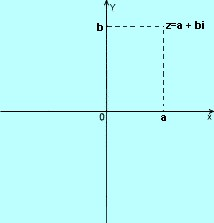
\includegraphics[width=0.5\textwidth]{wykres.jpg}
    \caption{Wykres $a+ib=z$}
    \label{fig:image1}
\end{figure}

, gdzie $a$ i $b$ są pewnymi liczbami rzeczywistymi oraz $i$ jest tzw. jednostką urojoną, tj. $i$ jest jednym z dwóch elementów zbioru liczb zespolonych, spełniającym warunek $i^2=-1$ (drugim elementem jest $-i$). Spotyka się czasami zapis $i=\sqrt{-1}$, który nie jest formalnie poprawny ze względu na fakt, że również $(-i)^2=-1$, jest on jednak uznawany za pewien skrót myślowy i powszechnie akceptowany.
\newpage
Postać $z=a+bi$ nazywana jest postacią algebraiczną (albo kanoniczną) liczby zespolonej z.\\
Dla liczby $z=a+bi$ definiuje się jej\\


    część rzeczywistą (łac. pars realis) jako $\mathrm{re}\;z = a$ (inne oznaczenia: $\Re z$,\, $\operatorname{Re}\, z$),
    
		część urojoną (łac. pars imaginaria) jako $\mathrm{im}\;z = b$ (inne oznaczenia: $\Im z$,\, $\operatorname{Im}\, z$).
\\

Przykładowo liczba $7 - 5i$ jest liczbą zespoloną, której część rzeczywista wynosi $7$, a część urojona $-5$. Liczby rzeczywiste są utożsamiane z liczbami zespolonymi o części urojonej równej $0$.
\\\\
Liczby postaci $z = 0 + bi$ nazywa się liczbami urojonymi.

\begin{figure}[h]
    \centering
    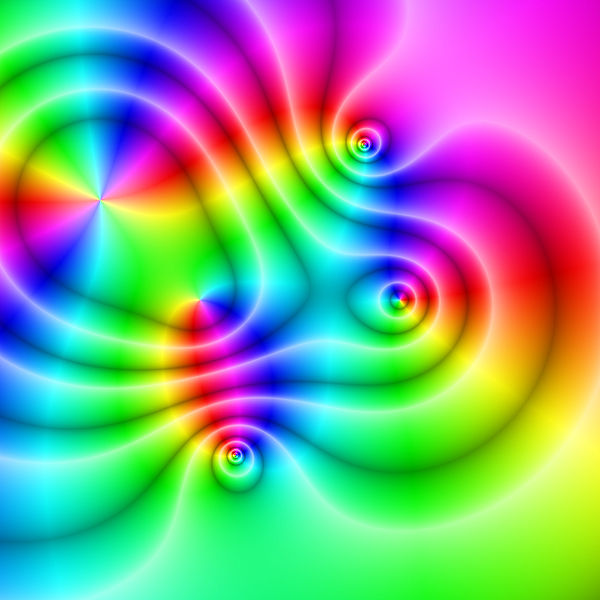
\includegraphics[width=0.5\textwidth]{matryca.jpg}
    \caption{Wykres}
    \label{fig:image}
\end{figure}

\begin{equation}
\label{eq:nr2}
	f(x) = \frac{(x^2-1)(x-2-i)^2}{(x^2+2+2i)}
\end{equation}

\vspace{0,3cm}

\subsection{Zadania:}
Zadanie 1.
\\\\
Udowodnij następujące własnosci dziań w zbiorze liczb zespolonych:
\\\\
a) $\forall z_1 , z_2 \in \mathbb{C} : z_1 + z_2 = z_2 + z_1$,\\
b) $\forall z_1 , z_2 , z_3 \in \mathbb{C} : (z_1 + z_2) + z_3 = z_1 + (z_2 + z_3)$,\\
c) $\forall z \in \mathbb{C} : z + 0 = z$, gdzie $0\stackrel{df}{=}(0, 0)$,\\
d) $\forall z \in \mathbb{C} : z - z = 0$,\\

\begin{picture}(40,30)
\put(40,30){\circle{11}}
\put(40,30){\circle{14}}
\put(15,10){\circle*{8}}
\put(20,10){\circle*{10}}
\put(30,20){\vector(1,0){30}}
\put(30,20){\vector(-4,1){30}}
\put(30,20){\vector(-1,4){5}}
\put(30,20){\vector(-1,-1){15}}
\put(30,20){\vector(-1,-4){5}}
\end{picture}

\newpage
\section{Macierze}
\subsection{Wstęp}
\label{sec:Wstep}

\subsubsection{Definicja}
\label{sec:Definicja}


\begin{center}\large {Macierze}
\end{center}
Macierz – w matematyce układ liczb, symboli lub wyrażeń zapisanych w postaci prostokątnej tablicy. Choć słowo „macierz” oznacza najczęściej macierz dwuwskaźnikową, to możliwe jest rozpatrywanie macierzy wielowskaźnikowych (zob. notacja wielowskaźnikowa). Macierze jednowskaźnikowe nazywa się często wektorami wierszowymi lub kolumnowymi, co wynika z zastosowań macierzy w algebrze liniowej. W informatyce macierze modeluje się zwykle za pomocą (najczęściej dwuwymiarowych) tablic. 
\cite{macierze}

\subsection{Wzory}
\label{sec:Wzory}

\begin{equation}
\label{eq:nr3}
\mathbf{X} =
\left( \begin{array}{ccc}
x_{11} & x_{12} & \ldots \\
x_{21} & x_{22} & \ldots \\
\vdots & \vdots & \ddots
\end{array} \right)
\end{equation}

\vspace{2cm}
\begin{table}[|h|]
\begin{tabular}{|l|l|l|l|l|l|}
  \hline 
  x & 0 & 1 & 2 & 3 & 4\\
  \hline
  0 & 0 & 0 & 0 & 0 & 0\\
  \hline
  1 & 0 & 1 & 2 & 3 & 4\\
  \hline
  2 & 0 & 2 & 4 & 1 & 3\\
  \hline
  3 & 0 & 3 & 1 & 4 & 2\\
  \hline
  4 & 0 & 4 & 3 & 2 & 1\\
  \hline
\end{tabular}
\end{table}

\vspace{2cm}
\begin{equation}
\label{eq:nr4}
\begin{cases}
a_{11}x_1 + a_{12}x_2 + \cdots + a_{1m}x_m = b_1 \\ 
a_{21}x_1 + a_{22}x_2 + \cdots + a_{2m}x_m = b_2 \\
\vdots\\
a_{n1}x_1 + a_{n2} x_2 + \cdots + a_{nm}x_m = b_n 
\end{cases} 
\end{equation}

\newpage

\bibliographystyle{unsrt}
\bibliography{biblio}

\end{document} 